\documentclass[12pt,oneside]{exam}

% This package simply sets the margins to be 1 inch.
\usepackage[margin=1in]{geometry}

% These packages include nice commands from AMS-LaTeX
\usepackage{amssymb,amsmath,amsthm,amsfonts,latexsym,verbatim,xspace,setspace}
\usepackage{hyperref}
\usepackage{graphicx}

% Make the space between lines slightly more
% generous than normal single spacing, but compensate
% so that the spacing between rows of matrices still
% looks normal.  Note that 1.1=1/.9090909...
\renewcommand{\baselinestretch}{1.1}
\renewcommand{\arraystretch}{.91}

% Define environments for exercises.
\newenvironment{exercise}[1]{\vspace{.1in}\noindent\textbf{Problem #1 \hspace{.05em}}}{}
\newenvironment{newsolution}{\vspace{.1in}\noindent\textbf{Solution: \hspace{.05em}}}{}

% define shortcut commands for commonly used symbols
\newcommand{\R}{\mathbb{R}}
\newcommand{\C}{\mathbb{C}}
\newcommand{\Z}{\mathbb{Z}}
\newcommand{\Q}{\mathbb{Q}}
\newcommand{\N}{\mathbb{N}}
\newcommand{\calP}{\mathcal{P}}
\DeclareMathOperator{\sech}{sech}
\DeclareMathOperator{\csch}{csch}
\DeclareMathOperator{\vsspan}{span}

\newcommand{\func}[3]{{#1} : {#2} \longrightarrow {#3}}

\title{Math 514 - Summer II 2020: Long Quiz 1}

%%%%%%%%%%%%%%%%%%%%%%%%%%%%%%%%%%%%%%%%%%

\begin{document}

\begin{flushright}
\sc MAT 514 - Summer II 2020\\
July 16, 2020
\end{flushright}
\bigskip
 
\begin{center}
\textsf{Solutions to Long Quiz 1} 
\end{center}

%%%%%%%%%%%%%%%%%%%%%%%%%%%%%%%%%%%%%%%%

\begin{exercise}{1}
Determine the real and imaginary parts\footnote{We will use the symbols $\Re(z), \Im(z)$ for the real and imaginary parts of a complex number $z$, respectively.} of the complex number 
\begin{equation*}
z = \frac{3i+2}{12+5i}
\end{equation*}
\end{exercise}

\textbf{Solution:} We begin by simplifying the expression, 
\begin{align*}
z & = \frac{3i+2}{12+5i} \\
& = \left(\frac{3i+2}{12+5i}\right)\left(\frac{12-5i}{12-5i}\right) \\
& = \frac{36i+15+24-10i}{169}\\
& = \frac{39+26i}{169}\\
& = \frac{3}{13} + \frac{2i}{13}
\end{align*}
Therefore the real and imaginary parts of $z$ are $\Re(z)=\frac{3}{13}$ and $\Im(z)=\frac{2}{13}$, respectively. 

\vfill
\begin{exercise}{2}
Find the conjugate, norm, and polar angle of the complex number
\begin{equation*}
z = \frac{4}{\sqrt{3}-i}
\end{equation*}
\end{exercise}

\textbf{Solution:} We begin by simplifying $z$, 
\begin{align*}
z & = \frac{4}{\sqrt{3}-i}\\
& = \left(\frac{4}{\sqrt{3}-i}\right)\left(\frac{\sqrt{3}+i}{\sqrt{3}+i}\right)\\
& = \frac{4\sqrt{3}+4i}{4}\\
& = \sqrt{3}+i.
\end{align*}
Its conjugate is $\overline{z} = \sqrt{3}-i$. Its norm is
\begin{equation*}
\|z\| = \sqrt{(\sqrt{3})^2 +(-1)^2} = 2. 
\end{equation*}

To find the polar angle, we write the complex number in polar form
\begin{equation*}
2(\cos(\theta)+i\sin(\theta)) = \sqrt{3}+i,
\end{equation*}
hence 
\begin{align*}
\cos(\theta) & = \frac{\sqrt{3}}{2},\\
\sin(\theta) & = \frac{1}{2},
\end{align*}
from which we infer $\theta = \frac{\pi}{6}$. 
\vfill


\begin{exercise}{3}
Sketch the set 
\begin{equation*}
\{z \in \C | \Re(z^2) \leq 0 \}
\end{equation*}
in the complex plane. Determine its basic topological properties: is it open, closed, or neither; bounded; compact; connected?
\end{exercise}

\textbf{Solution:} To better understand this region, we will express it in rectangular coordinates. Let $z=x+iy$, so that 
\begin{equation*}
z^2 = (x+iy)^2 = (x^2-y^2)+i(2xy),
\end{equation*}
so $\Re(z^2) = (x^2-y^2)$. 
The region is thus a cone, which we plot below for values of $\|x\|, \|y\| \leq 3$. 
\begin{center}
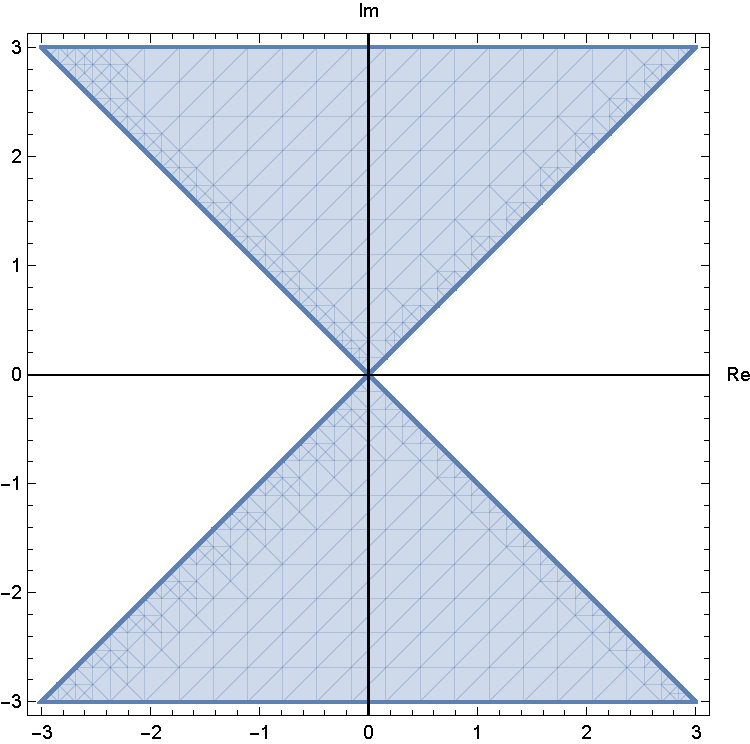
\includegraphics[scale=0.5]{p2.pdf} 
\end{center}
It is important to remark that this is not an entire plot, as the region is unbounded. Its topological properties are:
\begin{itemize}
\item it is closed;
\item it is not bounded;
\item it is not compact;
\item it is connected.
\end{itemize}
\vfill 

\begin{exercise}{4}
Determine whether the limit below exists:
\begin{equation*}
\lim_{z \to (1-i)} \Re(z)+i(2\Re(z) + \Im(z)).
\end{equation*}
If it exists, compute it. Otherwise, explain why it does not exist. 
\end{exercise}

\textbf{Solution:} The real and imaginary part functions are continuous, therefore, the limits may be computed by substitition:
\begin{align*}
\lim_{z \to (1-i)} \Re(z)+i(2\Re(z) + \Im(z)) & = \Re(1-i) +i(2\Re(1-i)+\Im(1-i))\\
& = 1+i(2-1)\\
& = 1+i.
\end{align*}
\vfill
\end{document}

